% Set Theory Crash Course with Professor Setterson
% A humorous yet rigorous introduction to set theory
\documentclass[11pt,a4paper]{article}

% Package imports
\usepackage[utf8]{inputenc}
\usepackage[T1]{fontenc}
\usepackage{amsmath,amssymb,amsthm}
\usepackage{tikz}
\usepackage{xcolor}
\usepackage{geometry}
\usepackage{fancyhdr}
\usepackage{tcolorbox}
\usepackage{enumitem}
\usepackage{hyperref}
\usepackage{graphicx}
\usepackage{multicol}

% TikZ libraries
\usetikzlibrary{shapes,arrows,positioning,calc,patterns,decorations.pathmorphing,backgrounds}

% Page setup
\geometry{margin=1in}
\pagestyle{fancy}
\fancyhead[L]{Set Theory Crash Course}
\fancyhead[R]{Prof. Setterson}

% Custom colors
\definecolor{profblue}{RGB}{70,130,180}
\definecolor{setgreen}{RGB}{60,179,113}
\definecolor{warmred}{RGB}{220,20,60}
\definecolor{goldenyellow}{RGB}{255,215,0}

% Custom commands for set notation
\newcommand{\N}{\mathbb{N}}
\newcommand{\Z}{\mathbb{Z}}
\newcommand{\Q}{\mathbb{Q}}
\newcommand{\R}{\mathbb{R}}
\newcommand{\C}{\mathbb{C}}
\newcommand{\PS}[1]{\mathcal{P}(#1)}

% Theorem environments
\theoremstyle{definition}
\newtheorem{definition}{Definition}[section]
\newtheorem{theorem}{Theorem}[section]
\newtheorem{example}{Example}[section]
\newtheorem{exercise}{Exercise}[section]

% Professor speech bubble command
\newcommand{\profsays}[1]{%
\begin{tcolorbox}[colback=yellow!10,colframe=profblue,title=Prof. Setterson says:]
#1
\end{tcolorbox}
}

% Title
\title{\Huge \textbf{Set Theory Crash Course} \\ \Large with Professor Setterson \\ \normalsize A Humorous Journey Through Mathematical Sets}
\author{Illustrated and Explained by Prof. S. Etterson}
\date{\today}

\begin{document}

\maketitle

% Title page illustration - Professor Setterson introduction
\begin{center}
\begin{tikzpicture}[scale=1.2]
    % Professor body
    \draw[fill=profblue!30,thick] (0,-1) ellipse (0.8 and 1.2);

    % Professor head
    \draw[fill=peachpuff,thick] (0,1) circle (0.8);

    % Wild Einstein-like hair
    \foreach \angle in {120,140,160,180,200,220,240} {
        \draw[thick,decoration={snake,amplitude=0.5mm},decorate]
            (0,1) -- ++(\angle:1.2);
    }

    % Glasses
    \draw[thick] (-0.3,1.1) circle (0.25);
    \draw[thick] (0.3,1.1) circle (0.25);
    \draw[thick] (-0.05,1.1) -- (0.05,1.1);

    % Eyes
    \fill (0.3,1.1) circle (0.08);
    \fill (-0.3,1.1) circle (0.08);

    % Mustache
    \draw[thick,decoration={snake,amplitude=0.3mm},decorate]
        (-0.3,0.7) .. controls (-0.4,0.6) and (-0.5,0.6) .. (-0.6,0.65);
    \draw[thick,decoration={snake,amplitude=0.3mm},decorate]
        (0.3,0.7) .. controls (0.4,0.6) and (0.5,0.6) .. (0.6,0.65);

    % Bow tie
    \draw[fill=warmred,thick] (-0.3,-0.2) -- (-0.1,-0.1) -- (-0.3,0) -- cycle;
    \draw[fill=warmred,thick] (0.3,-0.2) -- (0.1,-0.1) -- (0.3,0) -- cycle;
    \draw[fill=warmred!80,thick] (-0.1,-0.15) rectangle (0.1,-0.05);

    % Arms
    \draw[thick] (-0.6,-0.5) -- (-1.2,-0.8) -- (-1.4,-0.6);
    \draw[thick] (0.6,-0.5) -- (1.2,-0.3) -- (1.5,-0.1);

    % Speech bubble
    \draw[thick,fill=yellow!20] (2.5,1) ellipse (2 and 0.8);
    \draw[thick,fill=yellow!20] (1.5,0.5) -- (1.2,0.2) -- (1.8,0.4);
    \node[align=center] at (2.5,1) {Welcome to the\\wonderful world\\of SETS!};
\end{tikzpicture}
\end{center}

\newpage

\tableofcontents

\newpage

\section{Introduction: Meet Your Guide}

\begin{center}
\begin{tikzpicture}
    % Simplified professor for inline use
    \node (prof) at (0,0) {
        \begin{tikzpicture}[scale=0.8]
            \draw[fill=profblue!30,thick] (0,-0.5) ellipse (0.4 and 0.6);
            \draw[fill=peachpuff,thick] (0,0.5) circle (0.4);
            \foreach \angle in {120,150,180,210,240} {
                \draw[thick,decoration={snake,amplitude=0.3mm},decorate]
                    (0,0.5) -- ++(\angle:0.6);
            }
            \draw[thick] (-0.15,0.55) circle (0.12);
            \draw[thick] (0.15,0.55) circle (0.12);
            \fill (0.15,0.55) circle (0.04);
            \fill (-0.15,0.55) circle (0.04);
            \draw[fill=warmred,thick] (-0.15,-0.1) -- (-0.05,-0.05) -- (-0.15,0) -- cycle;
            \draw[fill=warmred,thick] (0.15,-0.1) -- (0.05,-0.05) -- (0.15,0) -- cycle;
        \end{tikzpicture}
    };

    \node[right=1cm of prof,align=left,text width=10cm] {
        \textbf{Greetings, aspiring set theorists!} I am Professor Setterson,
        and I'll be your guide through the fascinating realm of set theory.
        I've been teaching sets for so long, I remember when the empty set was
        just a twinkle in Cantor's eye!

        \vspace{0.3cm}

        In this crash course, we'll explore everything from basic set notation
        to power sets, with plenty of visual aids and terrible math puns along
        the way. Buckle up!
    };
\end{tikzpicture}
\end{center}

\profsays{Remember: A set is like a mathematical bag of goodies. It doesn't care about order, and it definitely doesn't like duplicates. It's the Marie Kondo of mathematics -- if an element doesn't spark joy (uniqueness), it doesn't make it in twice!}

\section{Basic Concepts: What's in a Set?}

\subsection{Definition of a Set}

\begin{definition}
A \textbf{set} is a well-defined collection of distinct objects, called \textbf{elements} or \textbf{members}.
\end{definition}

We denote sets using capital letters like $A$, $B$, $C$, and elements using lowercase letters like $a$, $b$, $c$.

\begin{center}
\begin{tikzpicture}
    % Draw a set as a blob
    \draw[thick,fill=setgreen!20] (0,0) ellipse (2 and 1.5);
    \node at (0,1.8) {$A$};

    % Add elements
    \node[circle,fill=profblue,minimum size=0.3cm,label=below:$a$] at (-0.5,0.3) {};
    \node[circle,fill=warmred,minimum size=0.3cm,label=below:$b$] at (0.5,0.3) {};
    \node[circle,fill=goldenyellow,minimum size=0.3cm,label=below:$c$] at (0,-0.5) {};

    % Professor pointing
    \begin{scope}[shift={(3.5,0)}]
        \draw[fill=profblue!30,thick] (0,-0.3) ellipse (0.3 and 0.4);
        \draw[fill=peachpuff,thick] (0,0.3) circle (0.3);
        \draw[thick] (-0.1,0.35) circle (0.08);
        \draw[thick] (0.1,0.35) circle (0.08);
        \draw[thick] (-0.3,0) -- (-0.8,-0.2);
        \draw[thick,->] (-0.8,-0.2) -- (-1.5,0);
    \end{scope}

    \node[right] at (4,0) {\small "Look! $a \in A$"};
\end{tikzpicture}
\end{center}

\subsection{Set Notation}

There are several ways to represent sets:

\begin{enumerate}
    \item \textbf{Roster notation}: $A = \{1, 2, 3, 4, 5\}$
    \item \textbf{Set-builder notation}: $B = \{x \in \N : x < 6\}$
    \item \textbf{Descriptive}: $C$ is the set of all vowels in the English alphabet
\end{enumerate}

\begin{example}
Let's see these in action:
\begin{itemize}
    \item $V = \{a, e, i, o, u\}$ (roster notation for vowels)
    \item $E = \{x \in \Z : x = 2k \text{ for some } k \in \Z\}$ (even integers)
    \item $\emptyset = \{\}$ (the empty set -- my favorite!)
\end{itemize}
\end{example}

\profsays{The empty set $\emptyset$ is like my refrigerator after my teenage son visits -- technically it exists, but there's nothing in it!}

\subsection{Important Set Relationships}

\begin{center}
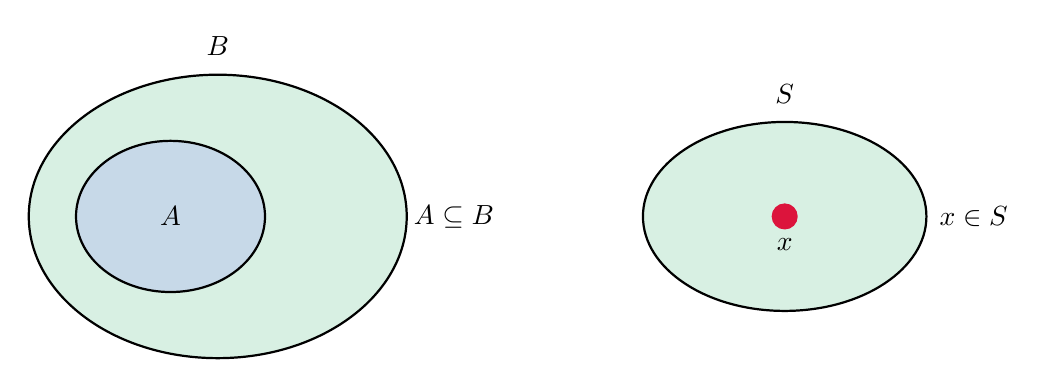
\begin{tikzpicture}[scale=1.2]
    % Subset illustration
    \draw[thick,fill=setgreen!20] (0,0) ellipse (2 and 1.5);
    \draw[thick,fill=profblue!30] (-0.5,0) ellipse (1 and 0.8);
    \node at (0,1.8) {$B$};
    \node at (-0.5,0) {$A$};
    \node at (2.5,0) {$A \subseteq B$};

    % Element membership
    \begin{scope}[shift={(6,0)}]
        \draw[thick,fill=setgreen!20] (0,0) ellipse (1.5 and 1);
        \node[circle,fill=warmred,minimum size=0.3cm] (elem) at (0,0) {};
        \node at (0,1.3) {$S$};
        \node at (0,-0.3) {$x$};
        \node at (2,0) {$x \in S$};
    \end{scope}
\end{tikzpicture}
\end{center}

\section{Subsets and Supersets}

\begin{definition}
Set $A$ is a \textbf{subset} of set $B$ (written $A \subseteq B$) if every element of $A$ is also an element of $B$.
\end{definition}

\begin{definition}
Set $A$ is a \textbf{proper subset} of set $B$ (written $A \subset B$) if $A \subseteq B$ and $A \neq B$.
\end{definition}

\begin{center}
\begin{tikzpicture}[scale=1.3]
    % Visual representation of subset relationships
    \draw[thick,fill=yellow!20] (0,0) ellipse (3 and 2);
    \draw[thick,fill=setgreen!30] (-0.8,0) ellipse (1.8 and 1.2);
    \draw[thick,fill=profblue!40] (-1.2,0) ellipse (0.8 and 0.6);

    \node at (0,2.3) {Universe $U$};
    \node at (-0.8,1.5) {$B$};
    \node at (-1.2,0) {$A$};

    % Professor explaining
    \begin{scope}[shift={(5,0)}]
        \draw[fill=profblue!30,thick] (0,-0.3) ellipse (0.3 and 0.4);
        \draw[fill=peachpuff,thick] (0,0.3) circle (0.3);
        \draw[thick] (-0.1,0.35) circle (0.08);
        \draw[thick] (0.1,0.35) circle (0.08);
        % Speech bubble
        \draw[thick,fill=yellow!20] (0,1.2) ellipse (1.5 and 0.5);
        \draw[thick,fill=yellow!20] (0,0.8) -- (-0.1,0.6) -- (0.1,0.7);
        \node[align=center,font=\footnotesize] at (0,1.2) {$A \subset B \subset U$};
    \end{scope}
\end{tikzpicture}
\end{center}

\profsays{Think of subsets like Russian nesting dolls -- each one fits perfectly inside the next, except in math, we can have dolls of the same size (when $A = B$, we have $A \subseteq B$ and $B \subseteq A$)!}

\section{Set Operations}

\subsection{Union}

\begin{definition}
The \textbf{union} of sets $A$ and $B$, denoted $A \cup B$, is the set of all elements that are in $A$ or $B$ (or both).
$$A \cup B = \{x : x \in A \text{ or } x \in B\}$$
\end{definition}

\begin{center}
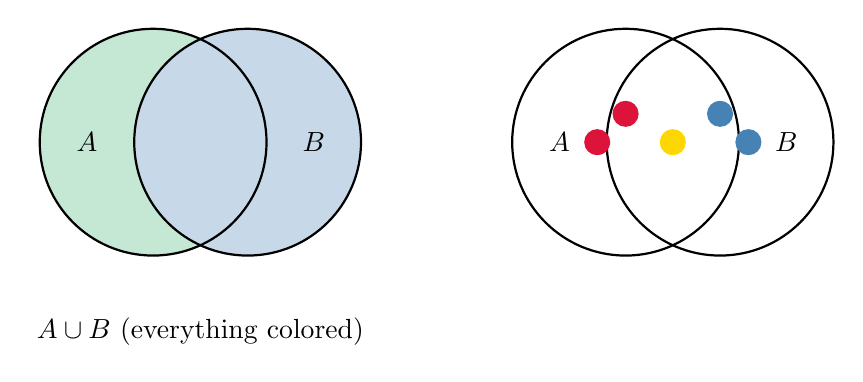
\begin{tikzpicture}[scale=1.2]
    % Union Venn diagram
    \begin{scope}
        \fill[setgreen!30] (-0.5,0) circle (1.2);
        \fill[profblue!30] (0.5,0) circle (1.2);
        \draw[thick] (-0.5,0) circle (1.2);
        \draw[thick] (0.5,0) circle (1.2);
        \node at (-1.2,0) {$A$};
        \node at (1.2,0) {$B$};
        \node at (0,-2) {$A \cup B$ (everything colored)};
    \end{scope}

    % Example with elements
    \begin{scope}[shift={(5,0)}]
        \draw[thick] (-0.5,0) circle (1.2);
        \draw[thick] (0.5,0) circle (1.2);
        \node[circle,fill=warmred,minimum size=0.2cm] at (-0.8,0) {};
        \node[circle,fill=warmred,minimum size=0.2cm] at (-0.5,0.3) {};
        \node[circle,fill=goldenyellow,minimum size=0.2cm] at (0,0) {};
        \node[circle,fill=profblue,minimum size=0.2cm] at (0.5,0.3) {};
        \node[circle,fill=profblue,minimum size=0.2cm] at (0.8,0) {};
        \node at (-1.2,0) {$A$};
        \node at (1.2,0) {$B$};
    \end{scope}
\end{tikzpicture}
\end{center}

\subsection{Intersection}

\begin{definition}
The \textbf{intersection} of sets $A$ and $B$, denoted $A \cap B$, is the set of all elements that are in both $A$ and $B$.
$$A \cap B = \{x : x \in A \text{ and } x \in B\}$$
\end{definition}

\begin{center}
\begin{tikzpicture}[scale=1.2]
    % Intersection Venn diagram
    \begin{scope}
        \fill[white] (-0.5,0) circle (1.2);
        \fill[white] (0.5,0) circle (1.2);
        \begin{scope}
            \clip (-0.5,0) circle (1.2);
            \fill[profblue!50] (0.5,0) circle (1.2);
        \end{scope}
        \draw[thick] (-0.5,0) circle (1.2);
        \draw[thick] (0.5,0) circle (1.2);
        \node at (-1.2,0) {$A$};
        \node at (1.2,0) {$B$};
        \node at (0,-2) {$A \cap B$ (overlap only)};
    \end{scope}

    % Professor with joke
    \begin{scope}[shift={(5,0)}]
        \draw[fill=profblue!30,thick] (0,-0.3) ellipse (0.3 and 0.4);
        \draw[fill=peachpuff,thick] (0,0.3) circle (0.3);
        \draw[thick] (-0.1,0.35) circle (0.08);
        \draw[thick] (0.1,0.35) circle (0.08);
        % Smiling mouth
        \draw[thick] (-0.1,0.2) arc (180:360:0.1);
    \end{scope}

    \node[align=center,text width=4cm] at (5,-1.5) {\footnotesize "The intersection is where\\sets have their meetings!"};
\end{tikzpicture}
\end{center}

\subsection{Set Difference}

\begin{definition}
The \textbf{difference} of sets $A$ and $B$, denoted $A \setminus B$ or $A - B$, is the set of elements in $A$ but not in $B$.
$$A \setminus B = \{x : x \in A \text{ and } x \notin B\}$$
\end{definition}

\begin{center}
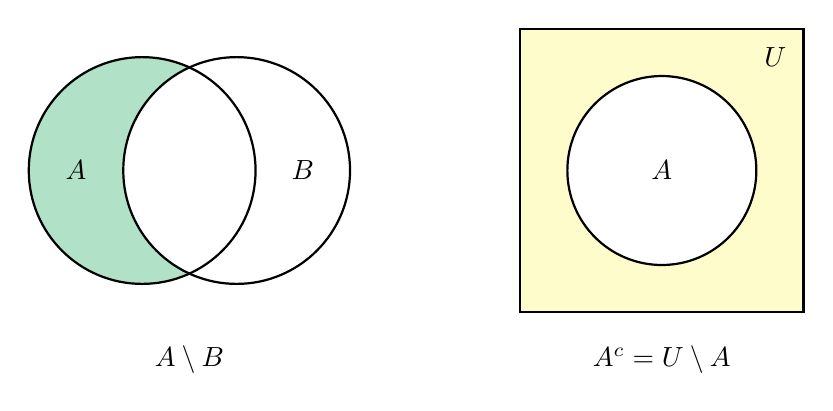
\begin{tikzpicture}[scale=1.2]
    % Set difference Venn diagram
    \begin{scope}
        \fill[setgreen!40] (-0.5,0) circle (1.2);
        \fill[white] (0.5,0) circle (1.2);
        \begin{scope}
            \clip (0.5,0) circle (1.2);
            \fill[white] (-0.5,0) circle (1.2);
        \end{scope}
        \draw[thick] (-0.5,0) circle (1.2);
        \draw[thick] (0.5,0) circle (1.2);
        \node at (-1.2,0) {$A$};
        \node at (1.2,0) {$B$};
        \node at (0,-2) {$A \setminus B$};
    \end{scope}

    % Complement illustration
    \begin{scope}[shift={(5,0)}]
        \draw[thick,fill=yellow!20] (-1.5,-1.5) rectangle (1.5,1.5);
        \draw[thick,fill=white] (0,0) circle (1);
        \node at (0,0) {$A$};
        \node at (1.2,1.2) {$U$};
        \node at (0,-2) {$A^c = U \setminus A$};
    \end{scope}
\end{tikzpicture}
\end{center}

\profsays{Set difference is like eating a cookie -- $A \setminus B$ is what's left of $A$ after $B$ takes a bite out of it!}

\subsection{Symmetric Difference}

\begin{definition}
The \textbf{symmetric difference} of sets $A$ and $B$, denoted $A \triangle B$, consists of elements in either $A$ or $B$ but not both.
$$A \triangle B = (A \setminus B) \cup (B \setminus A) = (A \cup B) \setminus (A \cap B)$$
\end{definition}

\section{Venn Diagrams: The Visual Language of Sets}

\begin{center}
\begin{tikzpicture}[scale=0.9]
    % Three-set Venn diagram
    \draw[thick,fill=red!20] (0,0) circle (1.5);
    \draw[thick,fill=blue!20,opacity=0.7] (1.2,0) circle (1.5);
    \draw[thick,fill=green!20,opacity=0.7] (0.6,1) circle (1.5);

    \node at (-0.8,-0.8) {$A$};
    \node at (2,-0.8) {$B$};
    \node at (0.6,2.2) {$C$};

    % Labels for regions
    \node[font=\tiny] at (0.6,0.3) {$A \cap B \cap C$};

    % Professor explaining
    \begin{scope}[shift={(5,0.5)}]
        \draw[fill=profblue!30,thick] (0,-0.3) ellipse (0.3 and 0.4);
        \draw[fill=peachpuff,thick] (0,0.3) circle (0.3);
        \draw[thick] (-0.1,0.35) circle (0.08);
        \draw[thick] (0.1,0.35) circle (0.08);
        % Pointer
        \draw[thick,->] (-0.3,0) -- (-1.5,0.3);
    \end{scope}

    \node[align=center,text width=3cm] at (5,-1) {\footnotesize "With 3 sets, we get\\8 distinct regions!"};
\end{tikzpicture}
\end{center}

\section{Cardinality: Size Matters!}

\begin{definition}
The \textbf{cardinality} of a finite set $A$, denoted $|A|$ or $\#A$, is the number of elements in $A$.
\end{definition}

\subsection{Finite vs. Infinite Sets}

\begin{center}
\begin{tikzpicture}
    % Finite set
    \draw[thick,fill=setgreen!20] (0,0) ellipse (1.5 and 1);
    \node at (0,1.3) {Finite Set};
    \foreach \x in {1,2,3,4,5} {
        \node[circle,fill=profblue,minimum size=0.2cm] at ({-0.7+0.35*\x},0) {\tiny \x};
    }
    \node at (0,-1.5) {$|A| = 5$};

    % Infinite set
    \begin{scope}[shift={(4,0)}]
        \draw[thick,fill=goldenyellow!20] (0,0) ellipse (1.5 and 1);
        \node at (0,1.3) {Infinite Set};
        \node at (-0.7,0) {\small $1, 2, 3, ...$};
        \node at (0,-1.5) {$|\N| = \aleph_0$};
    \end{scope}

    % Professor with infinity symbol
    \begin{scope}[shift={(8,0)}]
        \draw[fill=profblue!30,thick] (0,-0.3) ellipse (0.3 and 0.4);
        \draw[fill=peachpuff,thick] (0,0.3) circle (0.3);
        \draw[thick] (-0.1,0.35) circle (0.08);
        \draw[thick] (0.1,0.35) circle (0.08);
        % Holding infinity
        \draw[thick] (-0.3,-0.1) -- (-0.5,-0.3);
        \draw[thick] (0.3,-0.1) -- (0.5,-0.3);
        \node at (0,-0.5) {$\infty$};
    \end{scope}
\end{tikzpicture}
\end{center}

\profsays{Infinity isn't just a big number -- it's a concept! There are actually different sizes of infinity. Mind blown? Welcome to Cantor's paradise!}

\subsection{Cardinality Rules}

For finite sets $A$ and $B$:
\begin{itemize}
    \item $|A \cup B| = |A| + |B| - |A \cap B|$ (Inclusion-Exclusion Principle)
    \item $|A \times B| = |A| \cdot |B|$ (Cartesian Product)
    \item If $A \cap B = \emptyset$, then $|A \cup B| = |A| + |B|$
\end{itemize}

\section{Power Sets: Sets of Sets!}

\begin{definition}
The \textbf{power set} of a set $A$, denoted $\PS{A}$, is the set of all subsets of $A$, including the empty set and $A$ itself.
\end{definition}

\begin{theorem}
If $|A| = n$, then $|\PS{A}| = 2^n$.
\end{theorem}

\begin{example}
Let $A = \{1, 2, 3\}$. Then:
$$\PS{A} = \{\emptyset, \{1\}, \{2\}, \{3\}, \{1,2\}, \{1,3\}, \{2,3\}, \{1,2,3\}\}$$
Note that $|\PS{A}| = 8 = 2^3$.
\end{example}

\begin{center}
\begin{tikzpicture}[scale=0.8]
    % Power set visualization as a tree
    \node[circle,draw,thick] (empty) at (0,3) {$\emptyset$};

    \node[circle,draw,thick] (1) at (-3,1.5) {$\{1\}$};
    \node[circle,draw,thick] (2) at (0,1.5) {$\{2\}$};
    \node[circle,draw,thick] (3) at (3,1.5) {$\{3\}$};

    \node[circle,draw,thick] (12) at (-3,0) {$\{1,2\}$};
    \node[circle,draw,thick] (13) at (0,0) {$\{1,3\}$};
    \node[circle,draw,thick] (23) at (3,0) {$\{2,3\}$};

    \node[circle,draw,thick] (123) at (0,-1.5) {$\{1,2,3\}$};

    % Connections
    \draw[thick,->] (empty) -- (1);
    \draw[thick,->] (empty) -- (2);
    \draw[thick,->] (empty) -- (3);

    \draw[thick,->] (1) -- (12);
    \draw[thick,->] (1) -- (13);
    \draw[thick,->] (2) -- (12);
    \draw[thick,->] (2) -- (23);
    \draw[thick,->] (3) -- (13);
    \draw[thick,->] (3) -- (23);

    \draw[thick,->] (12) -- (123);
    \draw[thick,->] (13) -- (123);
    \draw[thick,->] (23) -- (123);

    \node at (0,4) {\textbf{Power Set Lattice}};

    % Professor amazed
    \begin{scope}[shift={(6,1)}]
        \draw[fill=profblue!30,thick] (0,-0.3) ellipse (0.3 and 0.4);
        \draw[fill=peachpuff,thick] (0,0.3) circle (0.3);
        % Wide eyes
        \draw[thick] (-0.1,0.35) circle (0.1);
        \draw[thick] (0.1,0.35) circle (0.1);
        \fill (-0.1,0.35) circle (0.05);
        \fill (0.1,0.35) circle (0.05);
        % Open mouth
        \draw[thick] (0,0.15) ellipse (0.08 and 0.05);
    \end{scope}

    \node[text width=3cm] at (6,-0.5) {\footnotesize "It forms a beautiful\\lattice structure!"};
\end{tikzpicture}
\end{center}

\profsays{The power set is like a set's family reunion -- everyone's invited, from the empty set (that weird uncle nobody talks about) to the full set itself!}

\section{Special Number Sets}

Here are the celebrity sets of mathematics:

\begin{center}
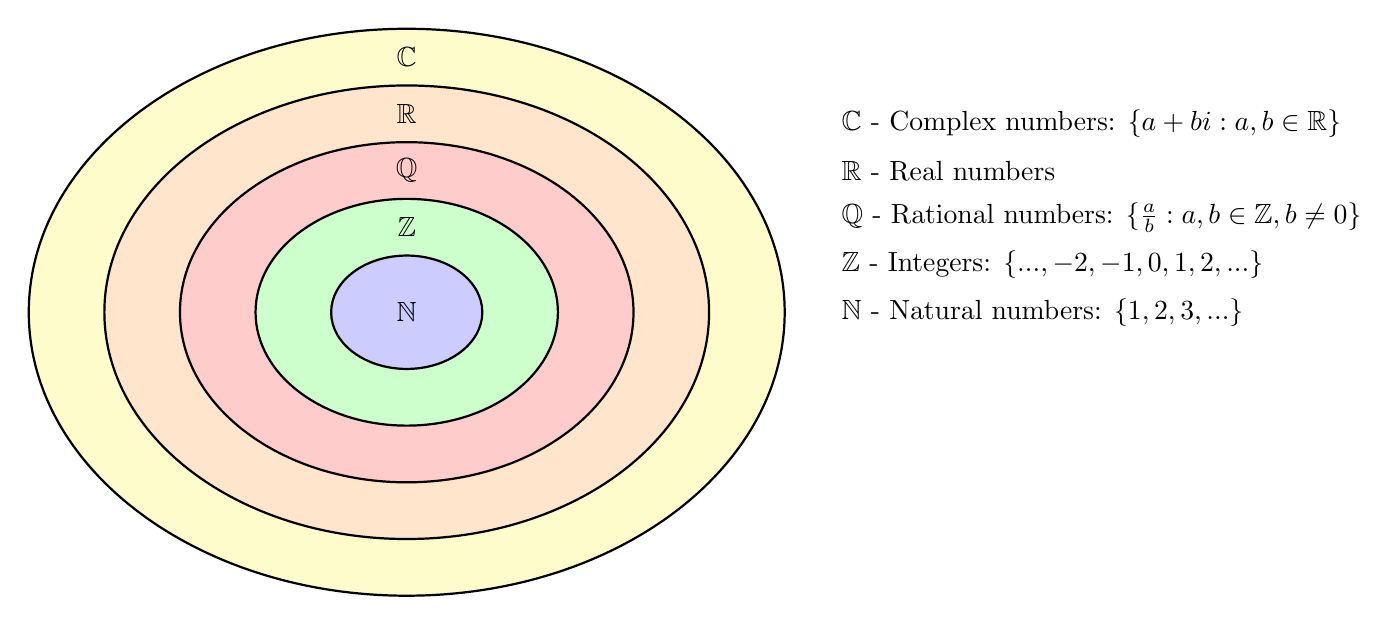
\begin{tikzpicture}[scale=1.2]
    % Nested number sets
    \draw[thick,fill=yellow!20] (0,0) ellipse (4 and 3);
    \draw[thick,fill=orange!20] (0,0) ellipse (3.2 and 2.4);
    \draw[thick,fill=red!20] (0,0) ellipse (2.4 and 1.8);
    \draw[thick,fill=green!20] (0,0) ellipse (1.6 and 1.2);
    \draw[thick,fill=blue!20] (0,0) ellipse (0.8 and 0.6);

    \node at (0,0) {$\N$};
    \node at (0,0.9) {$\Z$};
    \node at (0,1.5) {$\Q$};
    \node at (0,2.1) {$\R$};
    \node at (0,2.7) {$\C$};

    % Labels
    \node[right] at (4.5,0) {$\N$ - Natural numbers: $\{1, 2, 3, ...\}$};
    \node[right] at (4.5,0.5) {$\Z$ - Integers: $\{..., -2, -1, 0, 1, 2, ...\}$};
    \node[right] at (4.5,1) {$\Q$ - Rational numbers: $\{\frac{a}{b} : a, b \in \Z, b \neq 0\}$};
    \node[right] at (4.5,1.5) {$\R$ - Real numbers};
    \node[right] at (4.5,2) {$\C$ - Complex numbers: $\{a + bi : a, b \in \R\}$};
\end{tikzpicture}
\end{center}

\section{De Morgan's Laws}

\begin{theorem}[De Morgan's Laws]
For any sets $A$ and $B$:
\begin{align}
    (A \cup B)^c &= A^c \cap B^c\\
    (A \cap B)^c &= A^c \cup B^c
\end{align}
\end{theorem}

\begin{center}
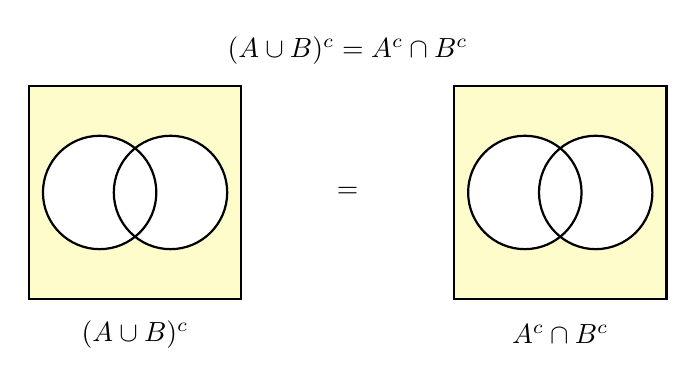
\begin{tikzpicture}[scale=0.9]
    % First law visualization
    \node at (0,2) {\textbf{$(A \cup B)^c = A^c \cap B^c$}};

    % Left side
    \begin{scope}[shift={(-3,0)}]
        \draw[thick,fill=yellow!20] (-1.5,-1.5) rectangle (1.5,1.5);
        \fill[white] (-0.5,0) circle (0.8);
        \fill[white] (0.5,0) circle (0.8);
        \draw[thick] (-0.5,0) circle (0.8);
        \draw[thick] (0.5,0) circle (0.8);
        \node at (0,-2) {$(A \cup B)^c$};
    \end{scope}

    \node at (0,0) {$=$};

    % Right side
    \begin{scope}[shift={(3,0)}]
        \draw[thick,fill=yellow!20] (-1.5,-1.5) rectangle (1.5,1.5);
        \fill[white] (-0.5,0) circle (0.8);
        \fill[white] (0.5,0) circle (0.8);
        \draw[thick] (-0.5,0) circle (0.8);
        \draw[thick] (0.5,0) circle (0.8);
        \node at (0,-2) {$A^c \cap B^c$};
    \end{scope}
\end{tikzpicture}
\end{center}

\profsays{De Morgan was the party pooper of set theory -- he figured out how to negate everything! But seriously, these laws are incredibly useful in logic and computer science.}

\section{Exercises: Test Your Set Skills!}

\begin{exercise}
Let $A = \{1, 2, 3, 4\}$ and $B = \{3, 4, 5, 6\}$. Find:
\begin{enumerate}[label=(\alph*)]
    \item $A \cup B$
    \item $A \cap B$
    \item $A \setminus B$
    \item $B \setminus A$
    \item $A \triangle B$
\end{enumerate}
\end{exercise}

\begin{center}
\begin{tikzpicture}
    % Professor giving hints
    \draw[fill=profblue!30,thick] (0,-0.3) ellipse (0.3 and 0.4);
    \draw[fill=peachpuff,thick] (0,0.3) circle (0.3);
    \draw[thick] (-0.1,0.35) circle (0.08);
    \draw[thick] (0.1,0.35) circle (0.08);
    % Winking
    \draw[thick] (0.1,0.35) -- (0.05,0.35) -- (0.15,0.35);

    % Hint bubble
    \draw[thick,fill=yellow!20] (2,0.5) ellipse (2.5 and 0.7);
    \draw[thick,fill=yellow!20] (0.5,0.2) -- (0.3,0) -- (0.7,0.1);
    \node[align=center,font=\small] at (2,0.5) {Hint: Draw a Venn diagram\\to visualize the sets!};
\end{tikzpicture}
\end{center}

\begin{exercise}
Prove that for any set $A$: $A \cup \emptyset = A$ and $A \cap \emptyset = \emptyset$.
\end{exercise}

\profsays{The empty set is the identity element for union and the absorbing element for intersection. It's like the number 0 in addition and multiplication!}

\begin{exercise}
If $|A| = 5$, $|B| = 8$, and $|A \cap B| = 3$, find $|A \cup B|$.
\end{exercise}

\begin{exercise}
Let $S = \{a, b\}$. Write out all elements of $\PS{S}$ and verify that $|\PS{S}| = 2^2 = 4$.
\end{exercise}

\begin{exercise}[Challenge]
Prove that for finite sets $A$, $B$, and $C$:
$$|A \cup B \cup C| = |A| + |B| + |C| - |A \cap B| - |A \cap C| - |B \cap C| + |A \cap B \cap C|$$
\end{exercise}

\begin{center}
\begin{tikzpicture}
    % Professor encouraging
    \draw[fill=profblue!30,thick] (0,-0.3) ellipse (0.3 and 0.4);
    \draw[fill=peachpuff,thick] (0,0.3) circle (0.3);
    \draw[thick] (-0.1,0.35) circle (0.08);
    \draw[thick] (0.1,0.35) circle (0.08);
    % Thumbs up
    \draw[thick] (0.3,-0.1) -- (0.5,0.1);
    \draw[thick] (0.5,0.1) -- (0.5,0.3);
    \draw[thick] (0.45,0.15) -- (0.45,0.25);

    \node[align=center,text width=6cm] at (3,0) {
        "This one's tricky! Think about\\
        overlapping regions in a three-set\\
        Venn diagram. You're counting\\
        some regions multiple times!"
    };
\end{tikzpicture}
\end{center}

\section{Cartesian Products}

\begin{definition}
The \textbf{Cartesian product} of sets $A$ and $B$, denoted $A \times B$, is the set of all ordered pairs $(a, b)$ where $a \in A$ and $b \in B$.
$$A \times B = \{(a, b) : a \in A \text{ and } b \in B\}$$
\end{definition}

\begin{example}
If $A = \{1, 2\}$ and $B = \{x, y, z\}$, then:
$$A \times B = \{(1,x), (1,y), (1,z), (2,x), (2,y), (2,z)\}$$
\end{example}

\begin{center}
\begin{tikzpicture}[scale=0.8]
    % Grid representation
    \draw[thick,->] (0,0) -- (4,0) node[right] {$B$};
    \draw[thick,->] (0,0) -- (0,3) node[above] {$A$};

    % Grid points
    \foreach \x in {1,2,3} {
        \foreach \y in {1,2} {
            \node[circle,fill=profblue,minimum size=0.3cm] at (\x,\y) {};
        }
    }

    % Labels
    \node[below] at (1,0) {$x$};
    \node[below] at (2,0) {$y$};
    \node[below] at (3,0) {$z$};
    \node[left] at (0,1) {$1$};
    \node[left] at (0,2) {$2$};

    % Example point
    \node[circle,fill=warmred,minimum size=0.3cm] at (2,2) {};
    \draw[thick,->] (3.5,2.5) -- (2.2,2.1);
    \node at (4,2.5) {$(2,y)$};

    % Professor
    \begin{scope}[shift={(6,1.5)}]
        \draw[fill=profblue!30,thick] (0,-0.3) ellipse (0.3 and 0.4);
        \draw[fill=peachpuff,thick] (0,0.3) circle (0.3);
        \draw[thick] (-0.1,0.35) circle (0.08);
        \draw[thick] (0.1,0.35) circle (0.08);
    \end{scope}

    \node[text width=3cm] at (7,0) {\footnotesize "It's like a\\mathematical\\chess board!"};
\end{tikzpicture}
\end{center}

\profsays{The Cartesian product is named after René Descartes. Fun fact: $\R \times \R = \R^2$ gives us the coordinate plane! So every time you graph something, you're using Cartesian products!}

\section{Relations and Functions}

\begin{definition}
A \textbf{relation} $R$ from set $A$ to set $B$ is a subset of $A \times B$.
\end{definition}

\begin{definition}
A \textbf{function} $f: A \to B$ is a special relation where each element in $A$ is related to exactly one element in $B$.
\end{definition}

\begin{center}
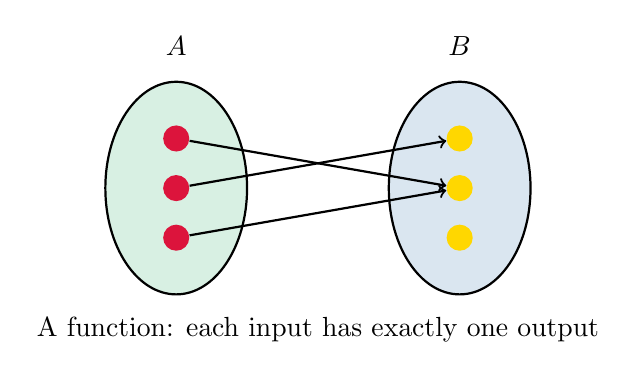
\begin{tikzpicture}[scale=0.9]
    % Function visualization
    \draw[thick,fill=setgreen!20] (-2,0) ellipse (1 and 1.5);
    \draw[thick,fill=profblue!20] (2,0) ellipse (1 and 1.5);

    \node at (-2,2) {$A$};
    \node at (2,2) {$B$};

    % Elements in A
    \node[circle,fill=warmred,minimum size=0.2cm] (a1) at (-2,0.7) {};
    \node[circle,fill=warmred,minimum size=0.2cm] (a2) at (-2,0) {};
    \node[circle,fill=warmred,minimum size=0.2cm] (a3) at (-2,-0.7) {};

    % Elements in B
    \node[circle,fill=goldenyellow,minimum size=0.2cm] (b1) at (2,0.7) {};
    \node[circle,fill=goldenyellow,minimum size=0.2cm] (b2) at (2,0) {};
    \node[circle,fill=goldenyellow,minimum size=0.2cm] (b3) at (2,-0.7) {};

    % Function arrows
    \draw[thick,->] (a1) -- (b2);
    \draw[thick,->] (a2) -- (b1);
    \draw[thick,->] (a3) -- (b2);

    \node at (0,-2) {A function: each input has exactly one output};
\end{tikzpicture}
\end{center}

\section{Advanced Topic: Countability}

\begin{definition}
A set is \textbf{countably infinite} if it can be put in one-to-one correspondence with $\N$.
\end{definition}

\begin{theorem}[Cantor's Diagonal Argument]
The set of real numbers $\R$ is uncountably infinite.
\end{theorem}

\begin{center}
\begin{tikzpicture}
    % Professor mind-blown
    \draw[fill=profblue!30,thick] (0,-0.3) ellipse (0.3 and 0.4);
    \draw[fill=peachpuff,thick] (0,0.3) circle (0.3);
    % Spiral eyes
    \draw[thick,decoration={coil,amplitude=0.5mm,segment length=1mm},decorate]
        (-0.1,0.35) circle (0.08);
    \draw[thick,decoration={coil,amplitude=0.5mm,segment length=1mm},decorate]
        (0.1,0.35) circle (0.08);

    % Explosion lines around head
    \foreach \angle in {0,30,60,90,120,150,180,210,240,270,300,330} {
        \draw[thick,orange] (0,0.8) -- ++(\angle:0.3);
    }

    \node[align=center,text width=6cm] at (3,0) {
        "There are more real numbers between 0 and 1\\
        than there are natural numbers in total!\\
        Different infinities! 🤯"
    };
\end{tikzpicture}
\end{center}

\section{Summary and Final Thoughts}

\begin{tcolorbox}[colback=profblue!10,colframe=profblue,title=Key Takeaways]
\begin{itemize}
    \item Sets are fundamental building blocks of mathematics
    \item Set operations (union, intersection, difference) follow specific rules
    \item Venn diagrams provide visual intuition for set relationships
    \item Power sets show the rich structure within sets
    \item Cardinality measures set size, even for infinite sets
    \item Set theory connects to functions, relations, and advanced mathematics
\end{itemize}
\end{tcolorbox}

\begin{center}
\begin{tikzpicture}[scale=1.5]
    % Final professor
    \draw[fill=profblue!30,thick] (0,-0.5) ellipse (0.4 and 0.6);
    \draw[fill=peachpuff,thick] (0,0.5) circle (0.4);
    \foreach \angle in {120,140,160,180,200,220,240} {
        \draw[thick,decoration={snake,amplitude=0.3mm},decorate]
            (0,0.5) -- ++(\angle:0.6);
    }
    \draw[thick] (-0.15,0.55) circle (0.12);
    \draw[thick] (0.15,0.55) circle (0.12);
    \fill (0.15,0.55) circle (0.04);
    \fill (-0.15,0.55) circle (0.04);

    % Graduation cap
    \draw[fill=black] (-0.3,0.9) -- (0.3,0.9) -- (0.3,1) -- (-0.3,1) -- cycle;
    \draw[fill=black] (0,1) ellipse (0.5 and 0.1);
    \draw[thick] (0,1) -- (0.3,1.2);
    \draw[fill=goldenyellow] (0.3,1.2) circle (0.05);

    % Arms up in celebration
    \draw[thick] (-0.3,-0.2) -- (-0.8,0.3);
    \draw[thick] (0.3,-0.2) -- (0.8,0.3);

    % Speech bubble
    \draw[thick,fill=yellow!20] (0,2) ellipse (2.5 and 0.6);
    \draw[thick,fill=yellow!20] (0,1.5) -- (-0.1,1.3) -- (0.1,1.4);
    \node[align=center] at (0,2) {Congratulations! You're now a\\Set Theory Scholar!};
\end{tikzpicture}
\end{center}

\profsays{Remember: In set theory, as in life, it's not about what you have, but how you organize it! Keep practicing, and soon you'll be seeing sets everywhere -- from database queries to probability theory. Until next time, may your sets be well-defined and your proofs be elegant!}

\section*{Solutions to Selected Exercises}

\begin{tcolorbox}[colback=green!10,colframe=green!50!black,title=Exercise 1 Solutions]
Given $A = \{1, 2, 3, 4\}$ and $B = \{3, 4, 5, 6\}$:
\begin{enumerate}[label=(\alph*)]
    \item $A \cup B = \{1, 2, 3, 4, 5, 6\}$
    \item $A \cap B = \{3, 4\}$
    \item $A \setminus B = \{1, 2\}$
    \item $B \setminus A = \{5, 6\}$
    \item $A \triangle B = \{1, 2, 5, 6\}$
\end{enumerate}
\end{tcolorbox}

\begin{tcolorbox}[colback=green!10,colframe=green!50!black,title=Exercise 3 Solution]
Using the inclusion-exclusion principle:
$$|A \cup B| = |A| + |B| - |A \cap B| = 5 + 8 - 3 = 10$$
\end{tcolorbox}

\vfill

\begin{center}
\textit{-- End of Crash Course --}\\
\small{Remember to practice with more problems and explore advanced topics!}
\end{center}

\end{document}